

\documentclass[twoside,twocolumn]{article}

\usepackage{blindtext} % Package to generate dummy text throughout this template 
\usepackage{graphicx}
\usepackage[sc]{mathpazo} % Use the Palatino font
\usepackage[T1]{fontenc} % Use 8-bit encoding that has 256 glyphs
\linespread{1.05} % Line spacing - Palatino needs more space between lines
\usepackage{microtype} % Slightly tweak font spacing for aesthetics

\usepackage[english]{babel} % Language hyphenation and typographical rules

\usepackage[hmarginratio=1:1,top=32mm,columnsep=20pt]{geometry} % Document margins
\usepackage[hang, small,labelfont=bf,up,textfont=it,up]{caption} % Custom captions under/above floats in tables or figures
\usepackage{booktabs} % Horizontal rules in tables

\usepackage{lettrine} % The lettrine is the first enlarged letter at the beginning of the text

\usepackage{enumitem} % Customized lists
\setlist[itemize]{noitemsep} % Make itemize lists more compact

\usepackage{abstract} % Allows abstract customization
\renewcommand{\abstractnamefont}{\normalfont\bfseries} % Set the "Abstract" text to bold
\renewcommand{\abstracttextfont}{\normalfont\small\itshape} % Set the abstract itself to small italic text

\usepackage{titlesec} % Allows customization of titles
\renewcommand\thesection{\Roman{section}} % Roman numerals for the sections
\renewcommand\thesubsection{\roman{subsection}} % roman numerals for subsections
\titleformat{\section}[block]{\large\scshape\centering}{\thesection.}{1em}{} % Change the look of the section titles
\titleformat{\subsection}[block]{\large}{\thesubsection.}{1em}{} % Change the look of the section titles

\usepackage{fancyhdr} % Headers and footers
\pagestyle{fancy} % All pages have headers and footers
\fancyhead{} % Blank out the default header
\fancyfoot{} % Blank out the default footer
\fancyhead[C]{DevOps en Base de Datos $\bullet$ Septiembre 2019 $\bullet$ } % Custom header text
\fancyfoot[RO,LE]{\thepage} % Custom footer text

\usepackage{titling} % Customizing the title section

\usepackage{hyperref} % For hyperlinks in the PDF

%----------------------------------------------------------------------------------------
%	TITLE SECTION
%----------------------------------------------------------------------------------------

\setlength{\droptitle}{-4\baselineskip} % Move the title up

\pretitle{\begin{center}\Huge\bfseries} % Article title formatting
\posttitle{\end{center}} % Article title closing formatting
\title{Mapeo Objeto Relacional} % Article title
\author{Sigfredo Aponte, Alonso Andia, Gabriela Atahuachi y Yhónn Condori}
\date{\today} % Leave empty to omit a date
\renewcommand{\maketitlehookd}{%
\begin{abstract}
\noindent 
En este artículo aprenderemos sobre el concepto y sus herramientas de mapeo objeto-relacional que nos permitirá crear una capa de acceso a los datos de una base de datos relacional, de tal forma que las tablas se transforman en clases y las filas de las tablas en objetos.\\
\textbf{Palabras clave:}   ORM, base de datos, herramientas, clases, objetos.\\
\end{abstract}
\begin{abstract}
\noindent 
In this article we learn about concept and tools of Object-Relational mapping ORM that we will allow us to create an access layer to the data of a relational database, in such a way that the tables are transformed into classes and the rows of the table into objects.\\
\textbf{Keywords:}   ORM, database, tools, classes, objects.
\end{abstract}
}
%----------------------------------------------------------------------------------------
\begin{document}
% Print the title
\maketitle
%----------------------------------------------------------------------------------------
%	ARTICLE CONTENTS
%----------------------------------------------------------------------------------------
\section{Introduccion}
\lettrine[nindent=0em,lines=3]{E}l mapeo relacional de objetos es una técnica que le permite consultar y manipular datos de una base de datos utilizando un paradigma orientad a objetos. Cuando se habla de ORM, la mayoría de personas se refieren a una biblioteca que implementa la técnica de mapeo relacional de objetos, de ahí la frase “un ORM”.
Una biblioteca ORM es una biblioteca completamente ordinaria escrita en su idioma de elección que encapsula el código necesario para manipular los datos, por lo que ya no usa SQL; interactúa directamente con un objeto en el mismo idioma que está utilizando.
.



%-------------------------------Marco Teórico-----------------

\section{Marco Teórico}
\subsection{Mapeo Objeto / Relacional}

El mapeo objeto-relacional es una técnica de programación para convertir datos del sistema de tipos utilizado en un lenguaje de programación orientado a objetos al utilizado en una base de datos relacional. En la práctica esto crea una base de datos virtual orientada a objetos sobre la base de datos relacional. Esto posibilita el uso de las características propias de la orientación a objetos (esencialmente la herencia y el polimorfismo)[1].

Las bases de datos relacionales solo permiten guardar tipos de datos primitivos (enteros, cadenas de texto, etc.) por lo que no se pueden guardar de forma directa los objetos de la aplicación en las tablas, sino que estos se deben de convertir antes en registros, que por lo general afectan a varias tablas. En el momento de volver a recuperar los datos, hay que hacer el proceso contrario, se deben convertir los registros en objetos. Es entonces cuando ORM cobra importancia, ya que se encarga de forma automática de convertir los objetos en registros y viceversa, simulando así tener una base de datos orientada a objetos [2].

\subsection{Estrategias de mapeo}

\subsubsection{Mapeo de herencia}
Las tres estrategias más comunes para representar un árbol de herencia de clases en un modelo relacional (en un RDBMS) son:
\begin{itemize}	
\item Mapeo filtrado
\item Mapeo horizontal
\item Mapeo vertical
\item Mapeo tabla genérica
\end{itemize} 
\subsubsection{Mapeo de relaciones}
\begin{itemize}	
\item Relación Uno-Uno
\item Relación Uno-Mucho
\item Relación Mucho-Mucho
\end{itemize} 
\subsubsection{Patrones de Diseño más conocidos}
\begin{itemize}	
\item Patrón Repository
\item Patrón Active Record
\end{itemize} 
\subsection{Ventajas del uso de ORM}
El utilizar el ORM nos puede proporcionar un grupo importante de ventajas:
\subsubsection{Rapidez en el desarrollo}
La mayoría de las herramientas actuales permiten la creación del modelo por medio del esquema de la base de datos, leyendo el esquema, nos crea el modelo adecuado.Una vez que se tiene el modelo creado, el programador irá mucho más rápido gracias a la metodología totalmente orientada a objetos, olvidándose así de las consultas a la base de datos[3].
\subsubsection{Abstracción de la base de datos}
Al utilizar un sistema ORM, lo que conseguimos es separarnos totalmente del sistema de base de datos que utilicemos y así, si en un futuro debemos de cambiar de motor de bases de datos, tendremos la seguridad de que este cambio no nos afectará a nuestro sistema, siendo el cambio mas sencillo.Todo sistema ORM debe de generar de forma automática las consultas a la base de datos para convertir los registros en objetos (y viceversa) y éstas deben poder adaptarse a los distintos proveedores (MySql, Oracle, PostreSQL,etc…), esto permitirá a los desarrolladores tener una preocupación menos a la hora de comenzar un proyecto, ya que tienen la seguridad de que un cambio drástico en el proveedor de base de datos, no impactará para nada en el tiempo de vida del proyecto[3].
\subsubsection{Reutilización}
Nos permite utilizar los métodos de un objeto de datos desde distintas zonas de la aplicación, incluso desde aplicaciones distintas[3].
\subsubsection{Seguridad}
Los ORM suelen implementar sistemas para evitar tipos de ataques como pueden ser los SQL injections. Inyección SQL es un método de infiltración de código intruso. Se dice que existe o se produjo una inyección SQL cuando, de alguna manera, se inserta o "inyecta" código SQL invasor dentro del código SQL programado, a fin de alterar el funcionamiento normal del programa y lograr así que se ejecute la porción de código "invasor", incrustado en la base de datos. Este tipo de intrusión normalmente es de carácter malicioso[3].
\subsubsection{Mantenimiento del código}
Nos facilita el mantenimiento del código debido a la correcta ordenación de la capa de datos[3].
\subsubsection{Lenguaje propio para realizar las consultas}
Estos sistemas de mapeo traen su propio lenguaje para hacer las consultas, lo que hace que los usuarios dejen de utilizar la sentencias
SQL para que pasen a utilizar el lenguaje propio de cada herramienta: Otra característica importante (de hecho seguramente la que más) es la exposición de clases y métodos que nos dan las herramientas ORM para poder extraer los datos de la forma que necesitemos
(filtros, ordenaciones, agrupaciones)[3].
\\
\\
\\
\\

%--------------------------------Fin Marco Teórico----------------

%-----------------------------------------------------------------
\section{Analisis}\label{sec:5}

En nuestro ejemplo usaremos la herramienta de Entity Framework.\\
\begin{itemize}
	\item En nuestra solucion SistemaGYM, tenemos dos proyectos que necesitamos para el mapeo.
		\begin{figure}[htb]
\begin{center}
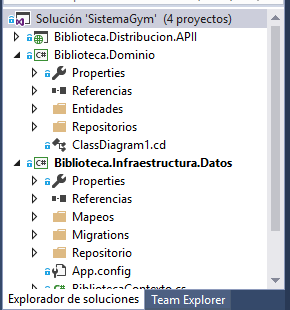
\includegraphics[width=5cm]{./Imagenes/1}
\end{center}
\end{figure}
	\item En el proyecto Biblioteca.Dominio, donde se encuentra la capa de entidades.
\begin{figure}[htb]
\begin{center}
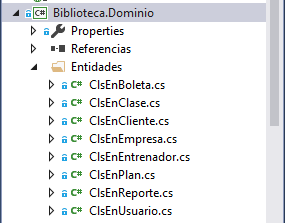
\includegraphics[width=5cm]{./Imagenes/2-1}
\end{center}
\end{figure}

	\item En cada clase se especifican los atributos y sus relaciones.
\begin{figure}[htb]
\begin{center}
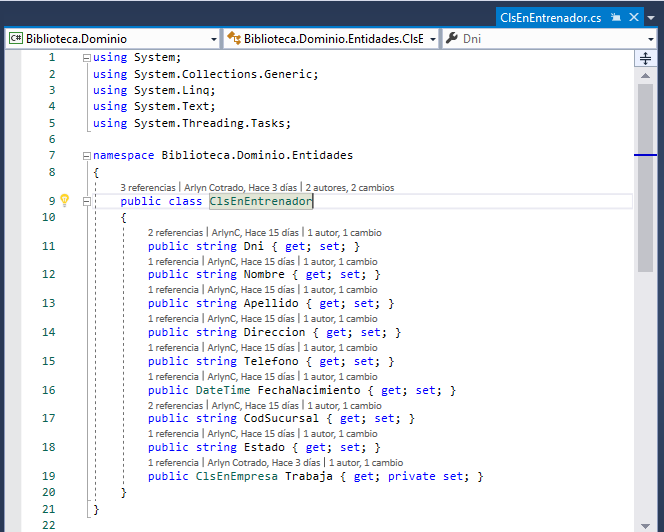
\includegraphics[width=7cm]{./Imagenes/2-2}
\end{center}
\end{figure}
\\
\\
\\
\\
\\
\\
\\
\\
\\
	\item En el proyecto Biblioteca.Infraestructura.Datos, donde se encuentran las tablas, relaciones y llaves.
\begin{figure}[htb]
\begin{center}
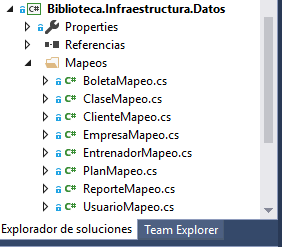
\includegraphics[width=5cm]{./Imagenes/3}
\end{center}
\end{figure}
\begin{figure}[htb]
\begin{center}
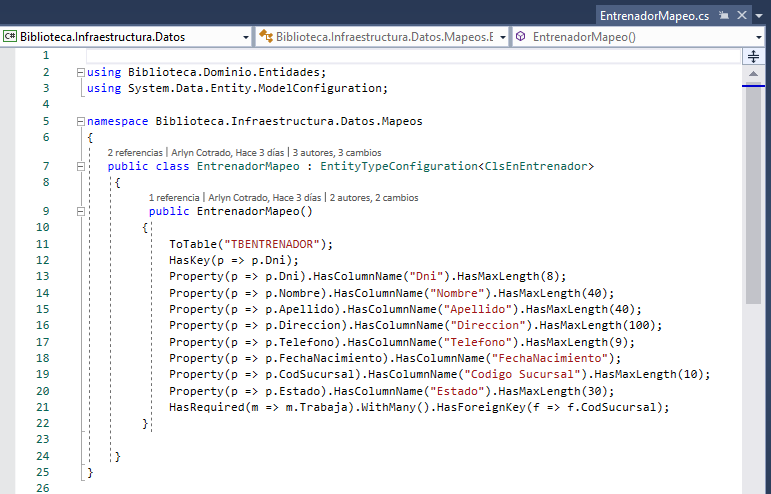
\includegraphics[width=8cm]{./Imagenes/3-1}
\end{center}
\end{figure}
\\
\\
\\
\\
\\
\\
\\
\\
\\
\\
\\
\\
\\
\\
\\
\\
\\
	\item Creamos el contexto de la base de datos.
\begin{figure}[htb]
\begin{center}
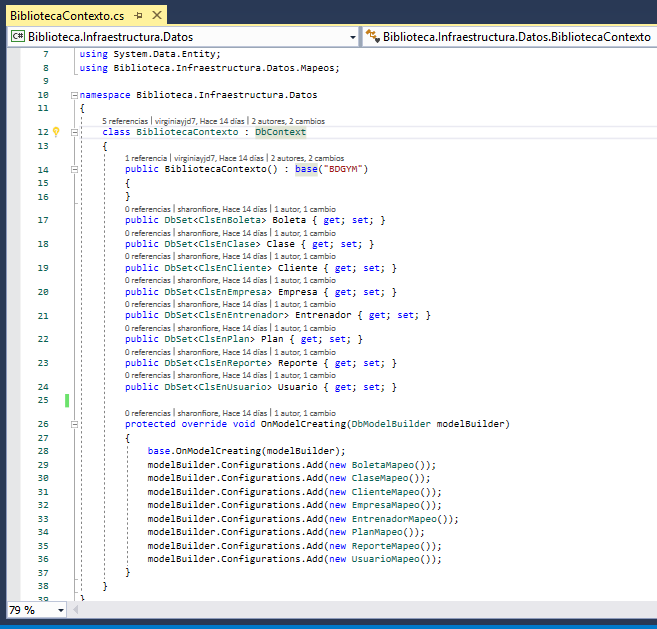
\includegraphics[width=7cm]{./Imagenes/4}
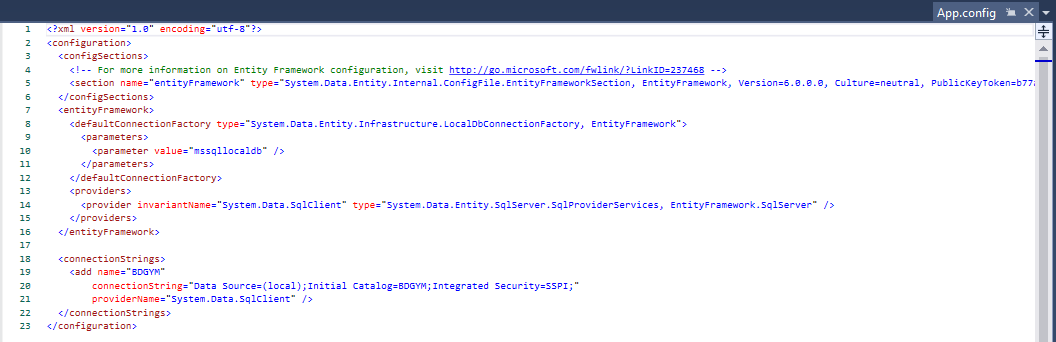
\includegraphics[width=8cm]{./Imagenes/4-1}
\end{center}
\end{figure}\\
\\
\\
\\
\\
\\
\\
\\
\\
\\
	\item Abrimos la Consola del Administrador de paquetes. Ingresamos los siguientes comandos: Enable-Migrations, add-migration, Update-Database.\\
\begin{figure}[htb]
\begin{center}
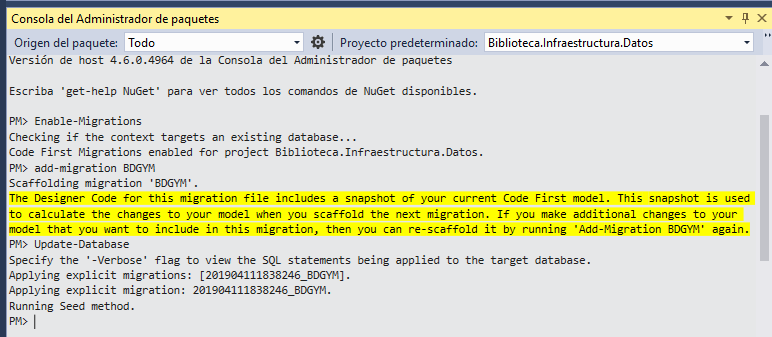
\includegraphics[width=8cm]{./Imagenes/5-1}
\end{center}
\end{figure}
	\item Por ultimo, vemos la base de datos, para ello entramos a SQL Server.
\begin{figure}[htb]
\begin{center}
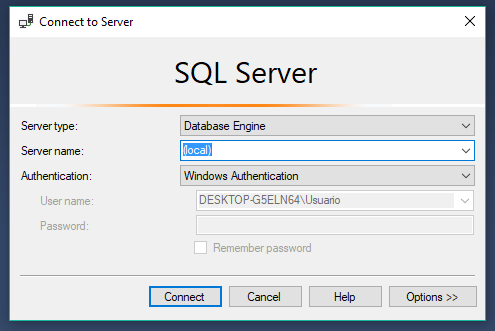
\includegraphics[width=6cm]{./Imagenes/5}
\end{center}
\end{figure}
\begin{figure}[htb]
\begin{center}
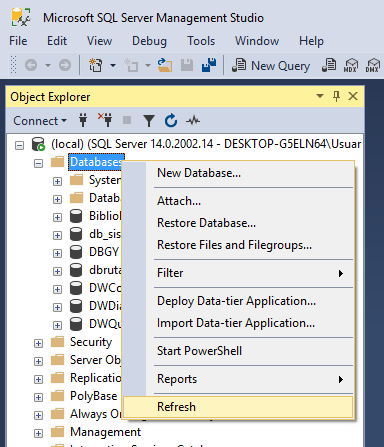
\includegraphics[width=5cm]{./Imagenes/5-2}
\end{center}
\end{figure}
\begin{figure}[htb]
\begin{center}
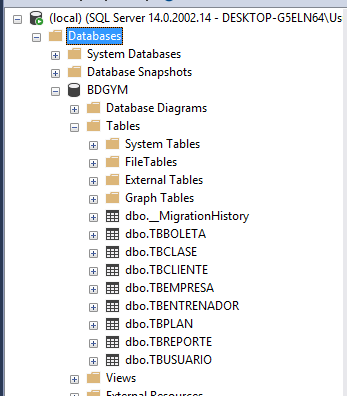
\includegraphics[width=6cm]{./Imagenes/5-3}
\end{center}
\end{figure}
\\
\\
\\
\\
\begin{figure}[htb]
\begin{center}
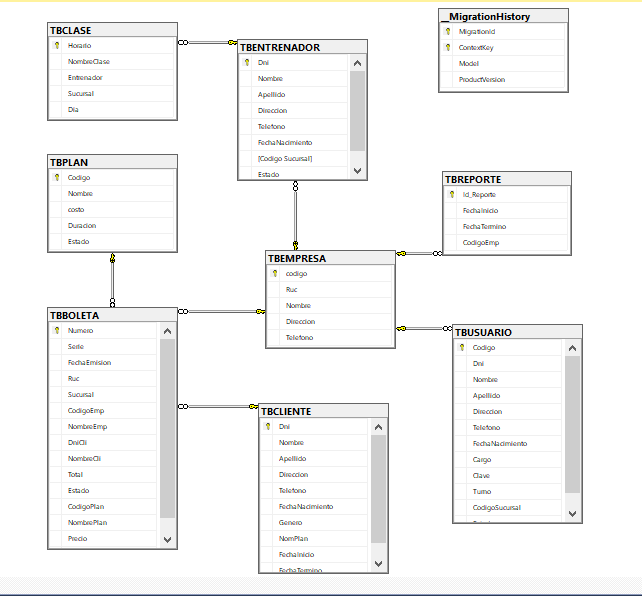
\includegraphics[width=7cm]{./Imagenes/6}
\end{center}
\end{figure}
\\
\\
\\
\\
\\
\\
\\
\\
\\
\\
\\
\end{itemize}


%-----------------------------------------------------------------


\section{Conclusiones}

ORM resuelve el desajuste del código objeto y la base de datos relacional con tres enfoques: de abajo hacia arriba, de arriba hacia abajo y se encuentran en el medio. Cada enfoque tiene su parte de beneficios y desventajas. Al seleccionar la mejor solución de software, los desarrolladores deben comprender completamente el entorno y los requisitos de diseño.




%	REFERENCE LIST
%----------------------------------------------------------------------------------------

\begin{thebibliography}{99} % Bibliography - this is intentionally simple in this template
\bibitem[1]{Osmel Yanes, Hansel Gracia:2011dg}
Osmel Yanes, Hansel Gracia (2011).
\newblock Mapeo Objeto / Relacional (ORM)
\bibitem[2]{Iván Guardado:2010dg}
Iván Guardado (2010).
\newblock  Introducción a Object-Relational Mapping (ORM)
\bibitem[3]{Fabiola Becerra, Elizabeth Hidalgo-Gato, Jesús Pérez:2009dg}
Fabiola Becerra, Elizabeth Hidalgo-Gato, Jesús Pérez (2009).
\newblock  OBJECT/RELATIONAL MAPPING
\bibitem[4]{SW Ambler:2010dg}
Ambler, SW (2010).
\newblock  Mapping objects to relational databases: O/R mapping in detail
 
 
\end{thebibliography}

%----------------------------------------------------------------------------------------


\end{document}
